\section{Analýza výsledků výzkumu}
Z jedenácti jedinců, kteří se výzkumu zúčastnili, oxymetr zaznamenal data osmi osob. Zbylá tři měření obsahovala prázdný soubor, což mohlo být způsobeno nesprávnou manipulací s oxymetrem - tato data musela být vyřazena. Z platných výsledků bylo 7 mužů a jedna žena, celkem 3 aktivní sportovci a 5 občasných sportovců. Kontrolní měření na jednom muži - občasném sportovci proběhlo úspěšně.
\subsection{Výsledky výzkumu}
\begin{figure}[ht]
\centering
  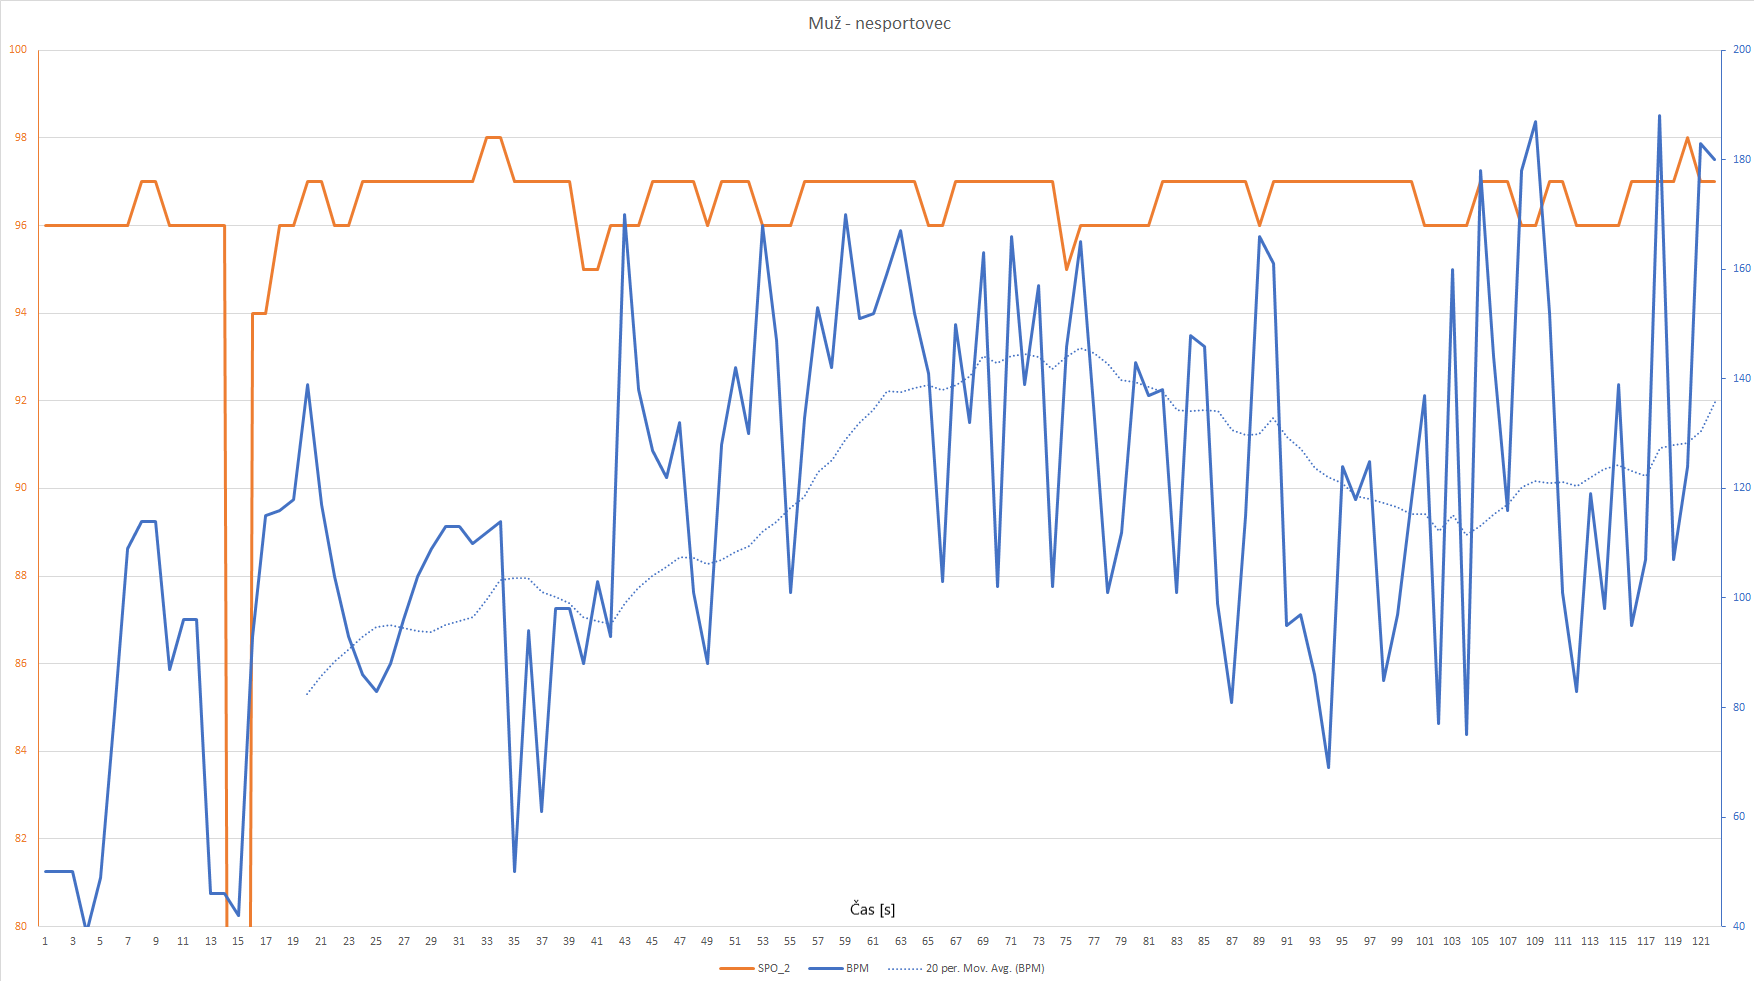
\includegraphics[scale=0.35, center]{Kapitoly/Prakticka/Obrazky/SpatnyGraf.png}
  \caption [Graf typického muže - nesportovce]{Většina výsledných grafů byla velmi podobná tomuto grafu jednoho z mužů - nesportovců; trend BPM byl celkově rostoucí, avšak v rámci sekund hodnoty oscilovaly s velkou amplitudou. Vliv tohoto krátkodobého cvičení na $SpO_2$ nebyl pozorován. Vlastní dílo}
  \label{fig:Spatny}
\end{figure}
Na většině výsledků lze, podobně jako na obrázku \ref{fig:Spatny}, vidět stoupající trend u tepové frekvence, nicméně okamžité hodnoty velmi výrazně oscilují, což je velmi pravděpodobně způsobeno chybou při měření. Také není možné dovodit žádný vztah mezi touto krátkodobou zátěží a $SpO_2$. Při měření $SpO_2$ také evidentně došlo k chybě, kdy oxymetr nezaznamenal tep a vyhodnotil saturaci jako 0\%.
\begin{figure}[ht]
\centering
  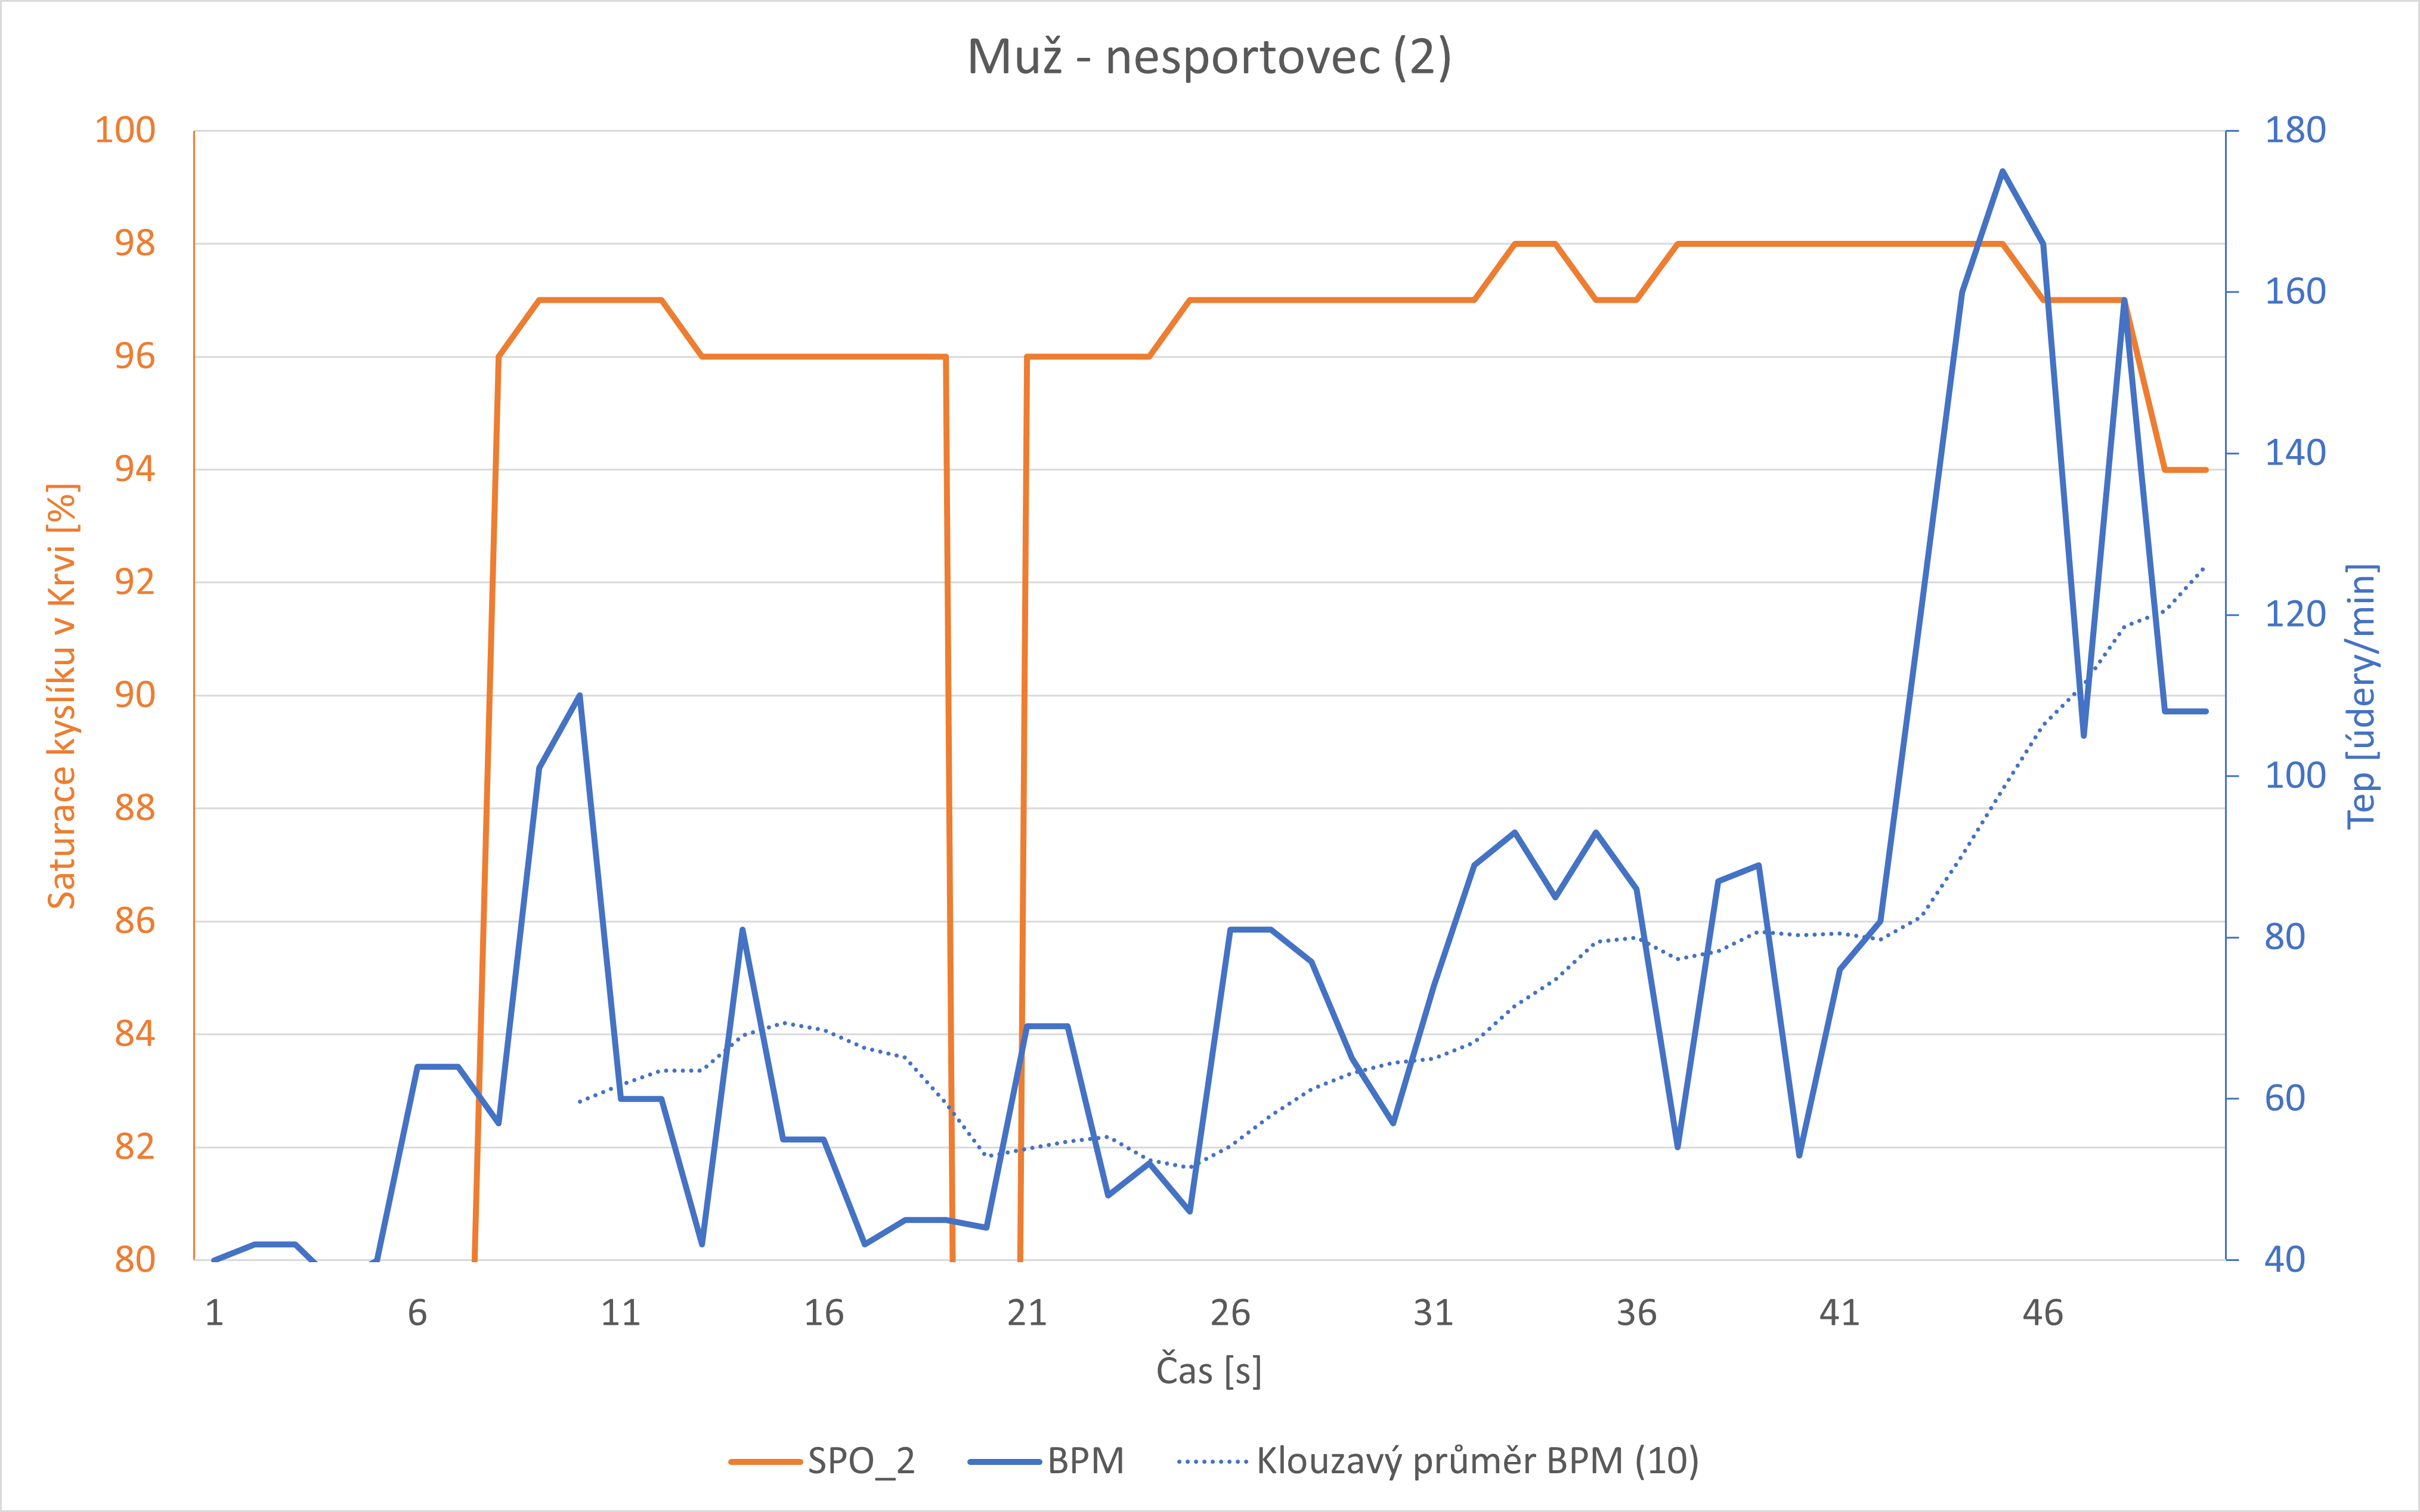
\includegraphics[scale=0.76, center]{Kapitoly/Prakticka/Obrazky/DobryGraf.png}
  \caption [Očekávaný graf muže - nesportovce]{Tento graf nejlépe demonstruje očekávané výsledky měření - BPM s časem (a tedy i námahou) roste, ke konci klesá saturace kyslíku v krvi. Vlastní dílo}
  \label{fig:Dobry}
\end{figure}
\par Obrázek \ref{fig:Dobry} ukazuje data, jež byla nejblíže naší hypotéze - tepová frekvence postupně roste (ačkoliv stále s oscilacemi), $SpO_2$ s rostoucí námahou a zadýcháváním ke konci naopak klesá. Je potřeba podotknout že se opravdu jedná o jediný graf, který naznačuje výrazněji tento trend.
\begin{figure}[ht]
\centering
  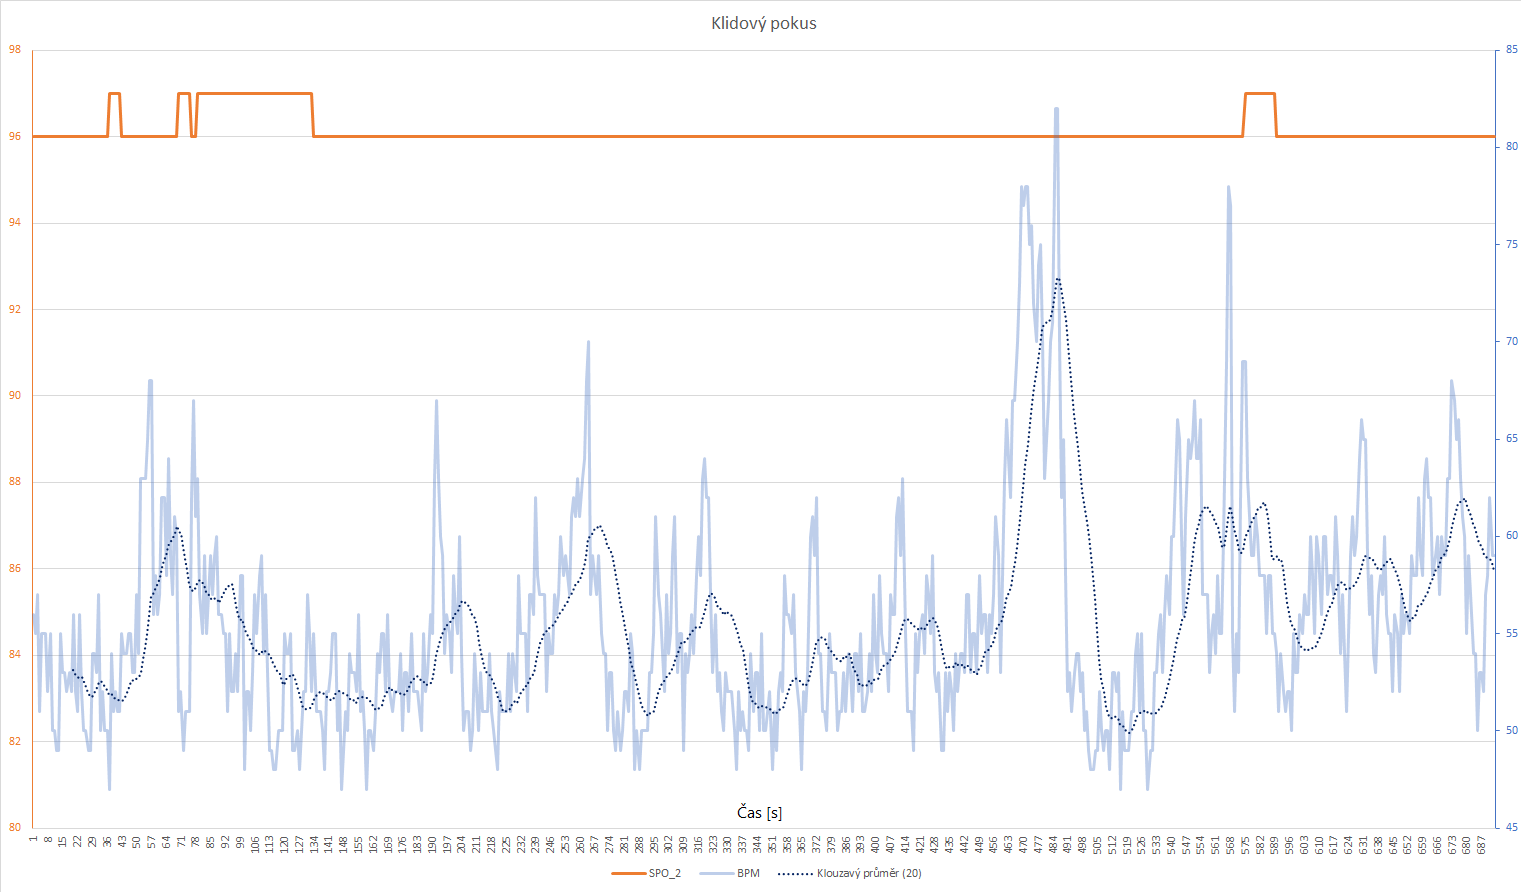
\includegraphics[scale=0.6, center]{Kapitoly/Prakticka/Obrazky/Kontrola.png}
  \caption [Kontrolní graf v klidu]{Kontrolní graf představuje nejpravděpodobnější využití našeho oxymetru - klidové měření ve středně dlouhých časových úsecích. Vlastní dílo}
  \label{fig:Control}
\end{figure}
\par Graf na obrázku \ref{fig:Control} konečně ukazuje naměřené hodnoty při středně dlouhém klidovém měření - lze vidět, že nedochází ke změnám saturace kyslíku v krvi, ani k výrazným změnám v naměřeném pulzu. Přesto jsou hodnoty, vzhledem k jejich vyšší stabilitě, reprezentativnější při zobrazení klouzavého průměru z posledních 20 hodnot. Dva úseky zvýšených hodnot na konci odpovídají zvýšené aktivitě vykonávané měřenou osobou.
\subsection{Diskuse}
Ačkoliv již bylo v práci mnohokrát zmíněno, že měření je pouze demonstrativní a není jeho cílem mít kvalitu vědeckého výzkumu (stejně, jako není cílem našeho oxymetru mít kvalitu certifikovaného zdravotnického zařízení), rozhodli jsme se zpětně zhodnotit průběh výzkumu a popsat jeho možné limitace a postřehy z měření, které by byly klíčové při opravdovém výzkumu.
\subsubsection{Možné limitace}
Jak zmiňují ve své práci například \cite{monitoring}, oxymetry nemají velkou přesnost při pohybu. U našeho konkrétního designu je velice pravděpodobné, že se při pohybu prst na samotném senzoru mohl pohybovat takovým způsobem, který senzor vyhodnotil jako tep a naměřil tedy vyšší BPM. BPM totiž oxymetr počítá nové při každém zaznamenaném tepu, a to jen z doby od tepu předchozího. To má tu výhodu, že jakýkoli falešný záznam o tepu ovlivní BPM jen na chvíli, a nechá ho vrátit na správnou hodnotu okamžitě po další dvojici reálných tepů. Nevýhodou ale je, že i bez falešných tepů výsledný graf BPM není naprosto konzistentní. Proto je vhodné jej proložit klouzavým průměrem.
\par Druhou potenciální limitací byl samotný typ cvičení, který nestanovoval žádné objektivní podmínky, což mohlo vést ke zkreslení některých dat, převážně u občasných sportovců, kteří mohli podat nižší, než maximální výkon.
\subsubsection{Metodika}
Kromě zapojení vyššího počtu účastníku, například i z jiných věkových kategorií, které by jistě pomohlo k tomu, aby tato demonstrace navíc přinesla zajímavá data, by jistě bylo vhodné měřit jednotlivé účastníky při více aktivitách různého typu. To by umožnilo docházet k závěrům ohledně vlivů jednotlivých typů cvičení na účastníky nebo by například mohlo pomoci určit případnou korelaci mezi změnou tepu a změnou saturace kyslíku. V tomto případě by samozřejmě bylo nutné kontrolní měření provést na všech účastnících, aby bylo možno odvozovat tyto vztahy.
\subsubsection{Shrnutí výsledků výzkumu}
Korelaci mezi tepovou frekvencí a fyzickou námahou se našemu přístroji v omezené míře povedlo demonstrovat, kdežto korelace mezi $SpO_2$ a námahou nebyla objevena. Jak se z grafů ukazuje, velikou výhodou pro využívání našeho oxymetru je využití delšího časového rozpětí pro vyhodnocování tepové frekvence (proložení grafu klouzavým průměrem). Díky tomu budou hodnoty nejen méně náchylné k náhodným prudkým změnám způsobených jedním špatným přečtením senzoru, ale i vhodnější pro sportovní využití, kde se vzhledem k pohybu dějí chyby na senzoru často a budou mít šanci se navzájem vyrušit, tak jak to bylo vidět u klouzavých průměrů na obrázcích \ref{fig:Spatny} a \ref{fig:Dobry}. Velikou výhodou našeho oxymetru je, že každý si bude moct vyhlazování dat klouzavým průměrem nastavit tak silné, jak bude pro konkrétní měření potřebovat.